\documentclass[a4paper,12pt]{article}
\newcounter{example}[]
\newenvironment{example}[1][]{\refstepcounter{example}\par\medskip
   \noindent \textbf{Example~\theexample. #1} \rmfamily}{\medskip}
   %%%%%%%%%%%%%%%%%%%%%%%%%%%%%%%%

%%%%%%%%%%%%%%%%%%%%%%%%%%%%%%%%%%
\usepackage[utf8]{inputenc}
\usepackage[english]{babel}
\usepackage{tikz-cd}
\usepackage{amsmath,amsfonts,amssymb,amsthm}
\usepackage{mathtools}
 \usepackage{float}
\usepackage{amsthm}
\usepackage{cite}
\usepackage{datetime} % British format dates
\usepackage[cm]{fullpage}
\usepackage{url}
\usepackage{hyperref}
\usepackage{stackrel,amssymb,amsmath}
\usepackage[nottoc]{tocbibind}
\usepackage{pgfplots}
\usepackage{rotating}
\usepackage[autostyle]{csquotes}
\usepackage{natbib}
\usepackage{graphicx}
\usepackage{natbib}
\usepackage{graphicx}

\newtheorem{problem}{Problem}
\newtheorem{attempt}{Attempt}
\newtheorem{question}{Question}


\newtheorem{theorem}{Theorem}[section]
\newtheorem{corollary}{Corollary}[theorem]
\newtheorem{lemma}[theorem]{Lemma}
\newtheorem{proposition}[theorem]{Proposition}
\theoremstyle{definition}
\newtheorem{definition}{Definition}[section]
\theoremstyle{indented}
\newtheorem*{remark}{Remark}
\newenvironment{titlemize}[1]{%
  \paragraph{#1}
  \begin{itemize}}
  {\end{itemize}}
  
  \usepackage[T1]{fontenc}
\usepackage{imakeidx}
\makeindex[columns=3, title=Alphabetical Index, intoc]
  
  
  %%%%%%%%%%5
\newcommand{\rightarrowdbl}{\rightarrow\mathrel{\mkern-14mu}\rightarrow}

\newcommand{\xrightarrowdbl}[2][]{%
  \xrightarrow[#1]{#2}\mathrel{\mkern-14mu}\rightarrow
}
%%%%%%%%%%%%%%5

\title{Region counting with mildly super-additive functions}
\author{Rhys Wells}
\date{\today}

\begin{document}

\maketitle
\tableofcontents

\section{Questions/Confusions/Tasks}


\section{Theory}

In studying the stability regions associated to universal fine compactified Jacobians there are two perspectives involved. The geometric perspective studying the space of polytopes, $P_n$ and the combinatorial perspective studying the function space $\tilde{P_n}$. We aim to examine the relationship between these spaces. Recall the geometric perspective.      
\begin{definition}\label{polytopes}
The space of polytopes is denoted by $P_n$, whose elements are the connected components of $\mathbb{R}^n \setminus  \cup H(S,k)$. The hyperplanes families 
$$H(S,k):= \left\{ \sum_{i\in S} x_i = k \right\}$$
are locally finite and have no accumulation point.
\end{definition}



For the function perspective we start with the integer valued set functions $\mathbb{Z}^{2^{[n]}}:=\{ f: 2^{[n]} \rightarrow \mathbb{Z}\}$ and we ask under what conditions are these functions related to $P_n$. For ease of notation let $\mathcal{P}_n ^{+} := 2^{[n]} \setminus \{\emptyset\}$.


\begin{definition} 
The function $f: \mathcal{P}_n ^{+}   \rightarrow \mathbb{Z}$ is mildly super additive (MSA) if for all $I,J \in  2^{[n]}$ with $I \cap J = \emptyset$ then 
$$0\le f(I \cup J) - f(I) -f(J) \le 1.$$


\begin{remark}(Possibility: Nimrod Megidoo: On finding additive, superadditive...)
  MSA functions are monotone increasing where $f(I)\le f(J)$ if $I \subseteq J$. Consider instead $f: \mathcal{P}_n ^{+}   \rightarrow \mathbb{Z}^{\ge 0}$ and set $f(\{\emptyset\})=0$. The sum function $\sum_{i \in S} x_i$ is an additive map. 
  \end{remark}

    \begin{definition}
    
    The space of mildly super additive functions is given by, $$\tilde{P_n}=\{ f: \mathcal{P}_n ^{+} \rightarrow \mathbb{Z} \mid f \text{ is mildly super-additive }\}.$$
    
    \end{definition}
    
    

\begin{remark}
     $\tilde{P_n}$ parameterises all fine compactified universal $g=1$ Jacobians (Check with preprint).
\end{remark}
    
       We now discuss two maps $\alpha: P_n \rightarrow \tilde{P_n}$ and $\beta:\tilde{P_n} \rightarrow P_n \cup \{\emptyset\}$ relating both spaces.
    
 \begin{definition}
 The map $\beta$ is given by $\beta:\tilde{P_n} &\rightarrow P_n \cup \{\emptyset\}$ is defined by
 
$$f \mapsto R_f= \bigcap_{S \in \mathcal{P}_{n}^{+}} \{\underline{x}\in \mathbb{R}^n \mid f(S) < \sum_{i \in S} x_i < f(S)+1\}.$$

 \end{definition}
 
 \begin{problem}
     The mildly super-additive condition can be shown to be necessary and sufficient condition for $R_f\ne \emptyset$, for $n=2,3,4$.
 \end{problem}

\begin{attempt}
google sheets file msa functions: Not necessarily true (the functions there are not msa so dont count). 
If you give me a function and its MSA is it empty? no , why not? is there enough space to be empty? see why the n=5 counterexample works. 
\end{attempt}

 \begin{example} For each $f \in \tilde{P_2}$, each region $R_f$ is given as the connected component of the following resonance diagram and integer translates.
   
   
      \begin{figure}[H]
    \centering
 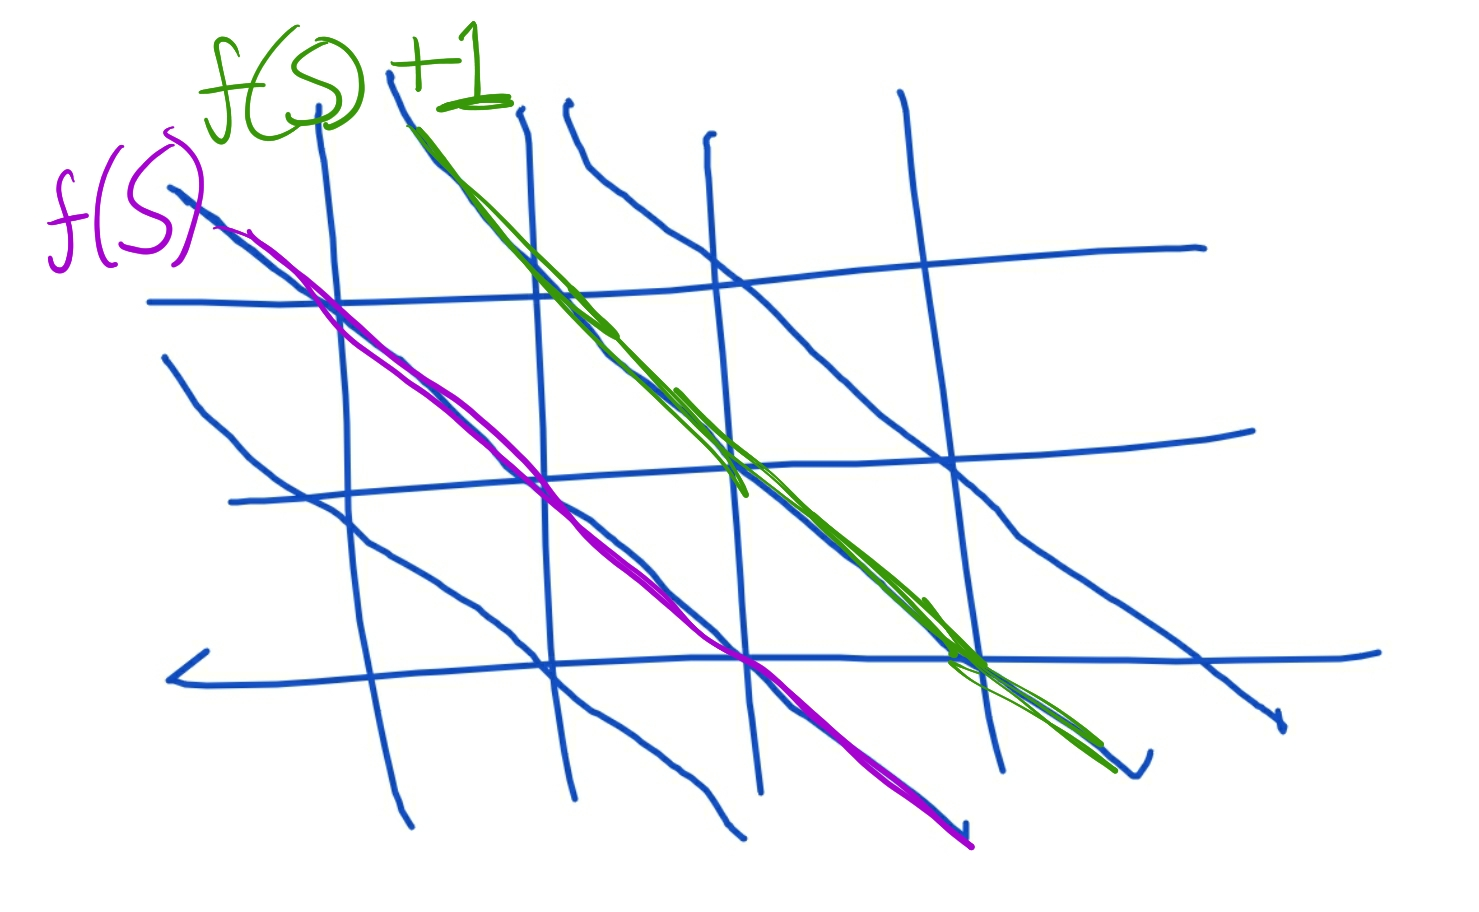
\includegraphics[scale=0.2,angle=0]{29072020 pics/translates.jpg}  
    \caption{}
    \label{translates}
\end{figure}
   
 \end{example}
 
 
 %%%%%%%%%%%%%%%%%%%%%%%%%%%%
 
 Note $\beta$ can map $f$ to $\emptyset$.
 
\begin{example}\label{counter}       

Let $n=5$ and consider $f \in \tilde{P_{5}}$ with $f(I)=0$ for $ I \nsupseteq \{ 1,3,5 \}$ or  $ I \nsupseteq \{ 2,4,5 \}$, and $f(I) = 1$ otherwise. Explicitly on $1$-sets and $2$-sets $f(I)=0$, on $f(\{1,3,5\})=f(\{2,4,5\})=1$ and on the other $3$-sets $f(I)=0$. On $4$-sets and $5$-sets $f(I)=1$. 
 
      
      This function is MSA. We check the MSA condition on each length of subset. For $1$-sets and $2$-sets it holds trivially. For a typical $3$-set such that $f(I)=0$ e.g. $f(\{2,3\}\sqcup \{5\})=0$ this is MSA by the $1$-set and $2$-set case, we also have $f(\{1,3\} \sqcup \{5\})=1$ which holds. For $4$-sets these decompose as a $3$-set and $1$-set or $2$-set and $2$-set. For a typical element e.g. $\{1,3,5,2\}$ we have $f(\{1,3,5\} \sqcup \{4\}) =1,2$ (where we can have either value $1$ or $2$), $f(\{1,3\} \sqcup \{5,4\})=0,1$ and $f(\{1,4,5\}\sqcup \{3\})=0,1$ the other decomposition's are of similar form so have a value of $1$ as the only possible choice and this agrees with the definition of $f$. Finally for $\{1,2,3,4,5\}$ we can write this as a $1$-set and $4$-set or $2$-set and $3$-set, with $f(\{1,2,3,4\} \sqcup \{5 \}) =1,2$ and $f(\{1,2 \}\sqcup \{3,4,5\}) =0,1$ and $f(\{1,3,5 \}\sqcup \{2,4\} ) =1,2$. Therefore the value is $1$ for the MSA condition to hold.
      
      We also see that $R_f=\emptyset$, as we have $1<x_1 + x_3 + x_5 <2$ and $0< x_2 +x_3 +x_5 <1$ and taking the difference gives $0<x_1 - x_2 <2$ which shows $x_1 > x_2$. Similarly take $0 < x_1 + x_4 + x_5 <1$ and $1 < x_2 +x_4 +x_5<2 $ and take the difference which gives $x_2 >x_1$ hence $R_f = \emptyset$ even if the mildly super additive condition holds. 
    \end{example}
    
    \begin{question}
What form does $f$ in this counterexample (Why is $R_f = \{\emptyset\}$ for $n=5$.)have compared to those that are MSA and those determined in $n=5$ case in Google sheet file. 
\end{question}

  
  \begin{remark}
       Regions of $P_n$ are defined by hyperplanes and inequalities. Hence each region gives for for each $S \in \mathcal{P}_n^{+}$ an integer.
  \end{remark}         
      
      \begin{definition}\label{alpha} Let $R \in P_n$ and $c \in \tilde{P_n}$ define the following map,
      
      \begin{align*}
          \alpha: P_n &\rightarrow \tilde{P_n}\\
          R &\mapsto c_R.
      \end{align*}
           
For $S \in 2^{[n] } \setminus \{\emptyset\} $ and  $\alpha (R)(S):=c_{R}(S)=c_{R,S}$. Let $\underline{x} \in R$ and set $c_{R,S}(\underline{x}) = Max \{ c \in \mathbb{Z} \mid c < \sum_{i \in S} x_i \}$.
   
      \end{definition}
         
\begin{example}
 
 To understand definition (\ref{alpha}) consider $n=2$. 

  \begin{figure}[H]
    \centering
 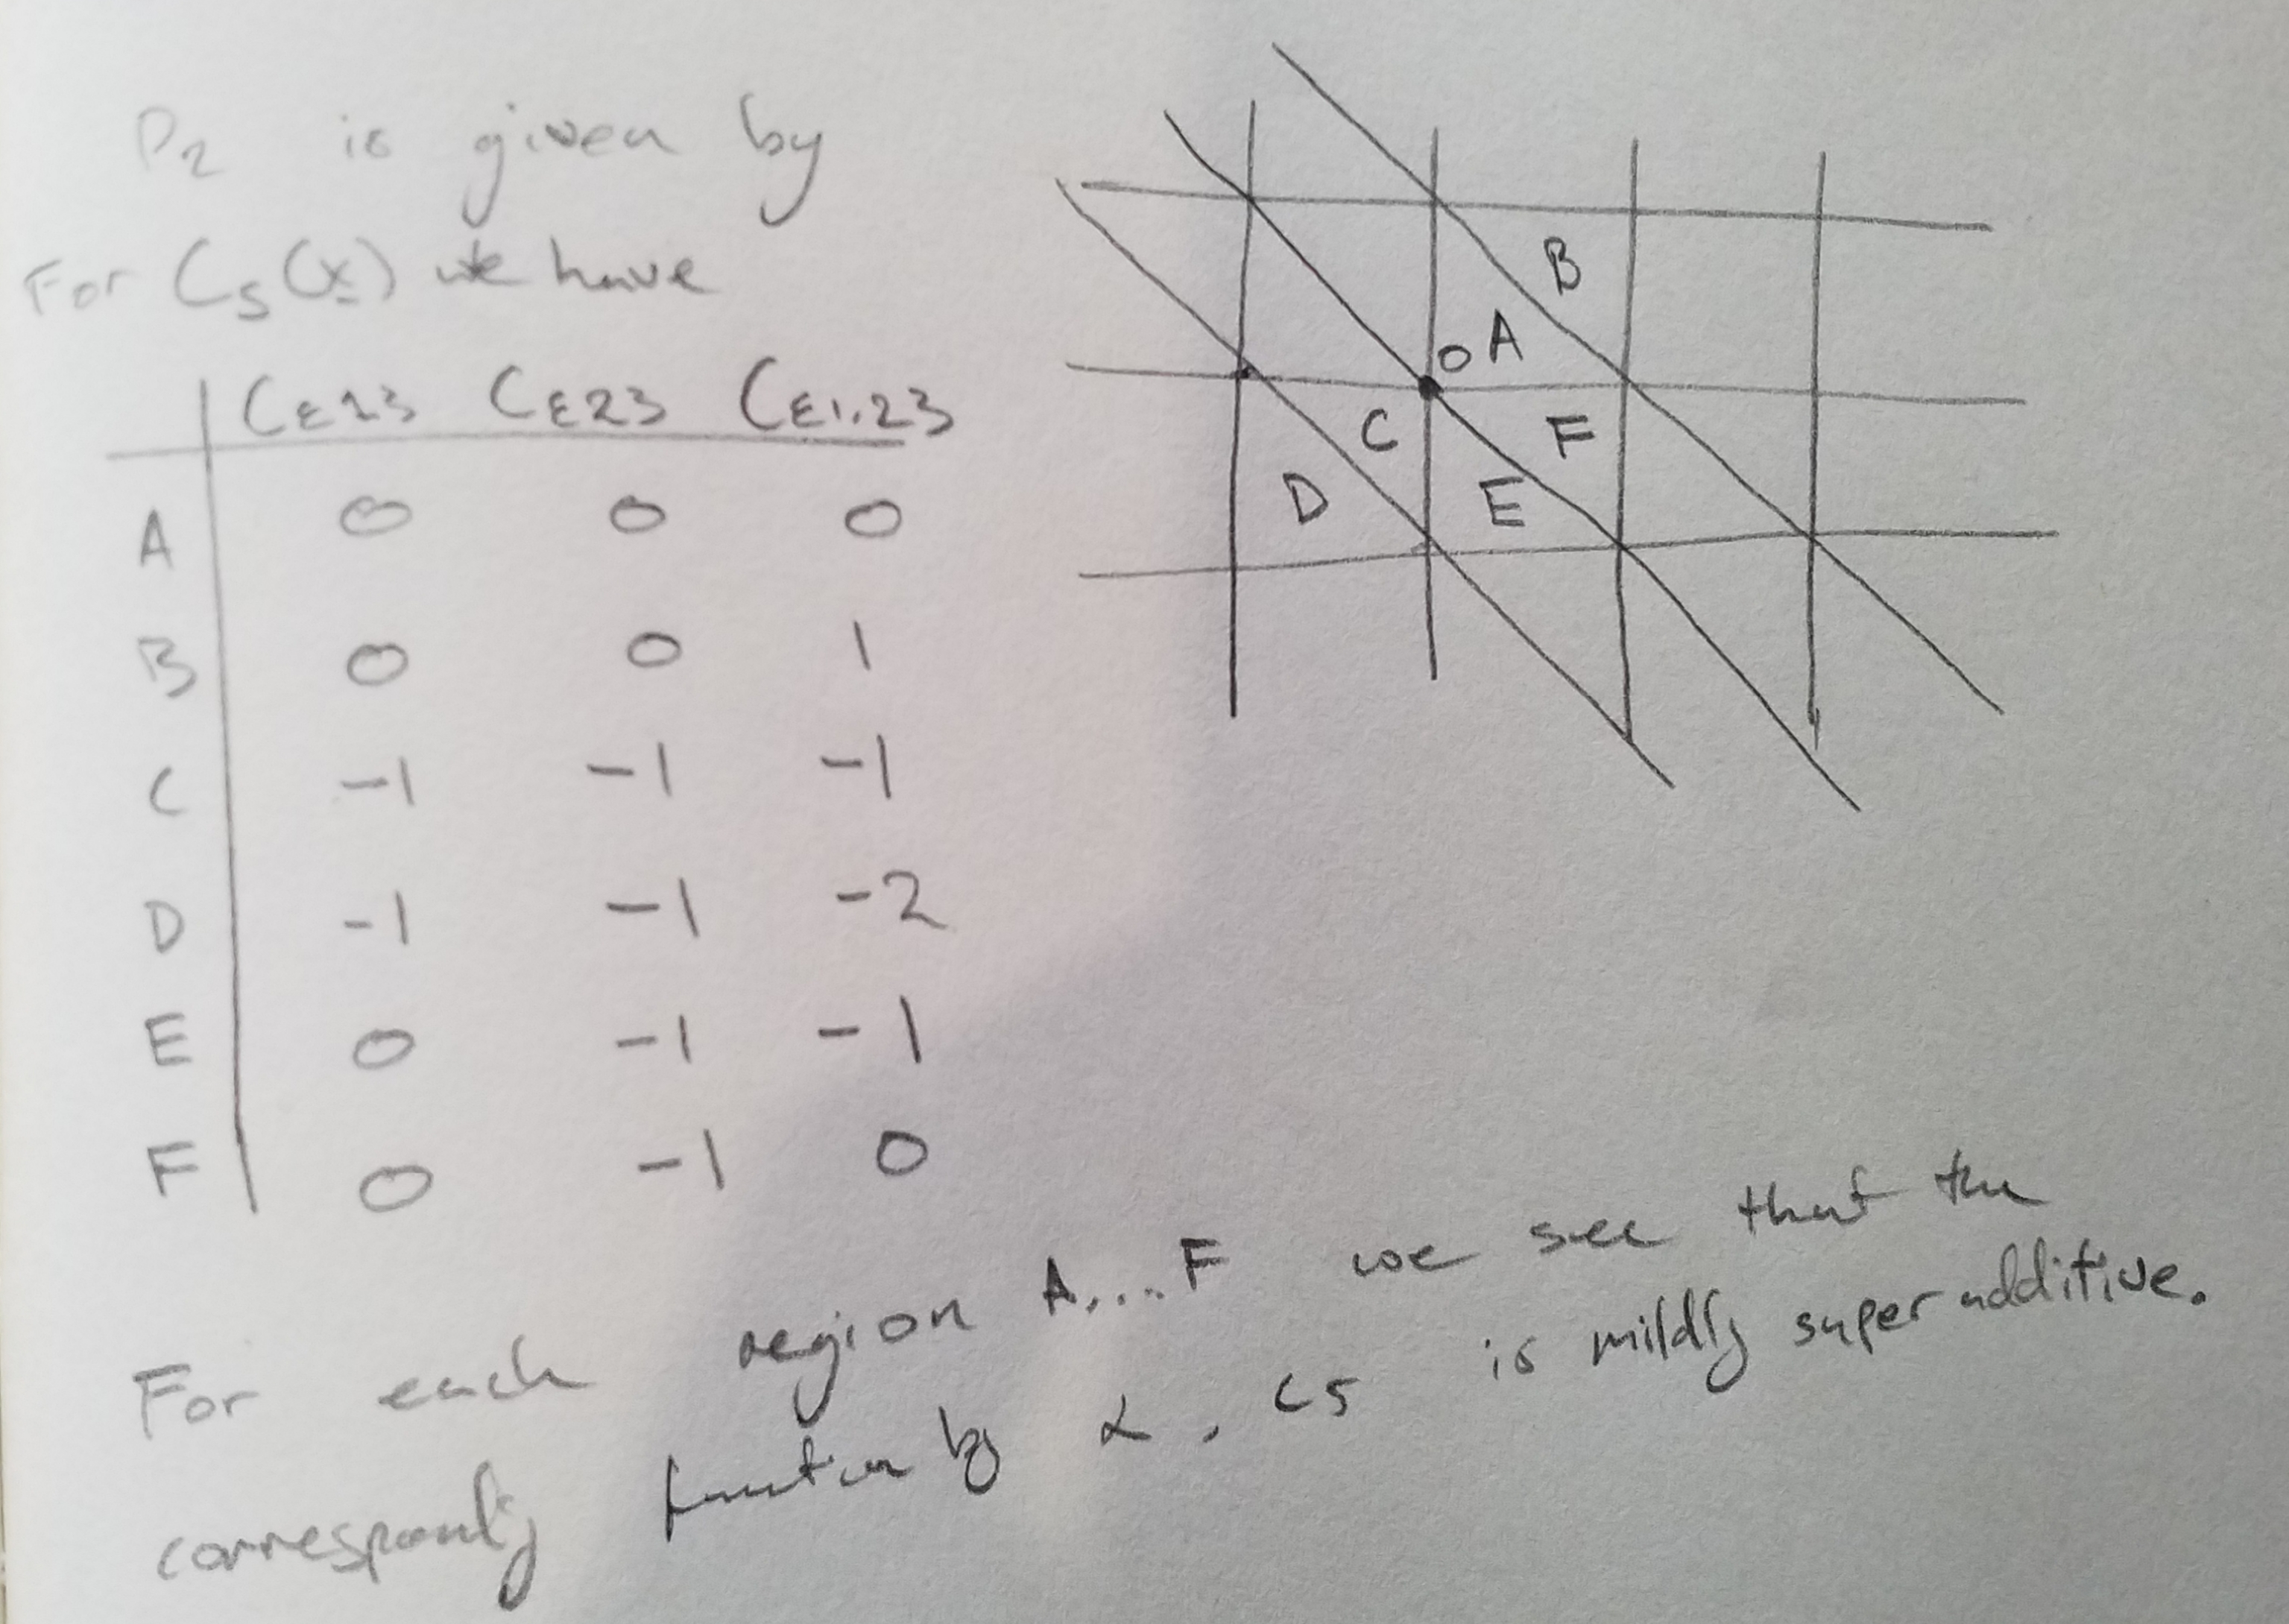
\includegraphics[scale=0.15,angle=0]{29072020 pics/fun meth Example.jpg}  
    \caption{}
    \label{relation}
\end{figure}
\end{example}

\begin{remark}\label{floor}
  Let $X_S:=\sum_{i \in S} x_i$ and recall the floor function. The function value for $c_{R,S}$ on $\underline{x} \in R$ can we written compactly as $c_{R,S}(\underline{x})=\lfloor X_S \rfloor$. Note the following inequalities for $\underline{x} \in R$,  $$\lfloor X_S \rfloor < X_S< \lceil X_S \rceil .$$ and $$\lfloor X_I \rfloor + \lfloor X_J \rfloor \le \lfloor X_{I \sqcup J} \rfloor <X_{I \sqcup J}  <\lceil X_{I \sqcup J} \rceil \le \lceil X_{I} \rceil + \lceil X_{J} \rceil   .$$
  
  
\end{remark}

For $\underline{x} \in R$, the function $c_{R,S}$ is independent of $\underline{x}$. On connected components $R \in P_n$ the floor function $c_{R,S}$ is continuous and discrete away from the boundary, hence $c_{R,S}$ constant. 

\begin{lemma}\label{msamap}
  For $R \in P_n$ the function $\alpha(R)=c_R:P_n^{+} \rightarrow \mathbb{Z}$ is mildly super additive. 
\end{lemma}

\begin{proof}
       Let $\underline{x} \in R$ by the definition of $H(S,k)$ one has $r < X_{I} < r+1$, $t<X_{J}<t+1$ and $k<X_{I \sqcup J}<k+1$. Take $r,t,k$ to be maximum otherwise the hyperplanes of $H(S,k)$ intersect $R$, contradicting the connected condition. Take the sum the first two inequalities to obtain 
       
       $$r+t<X_{I \sqcup J}<r+t+2,$$ 
   
   and compare this to $k<X_{I \sqcup J}<k+1$ to obtain $k<r+t+2$ and $r+t<k+1$. Hence $k-2<r+t<k+1$ and as $r+t \in \mathbb{Z}$ one has $r+t= k$ or $k-1$. In turn one has $k=r+t$ or $k=r+t+1$. Hence $\alpha(R)$ is mildly super additive.   
\end{proof}

  We conjecture the following set up shown in figure \ref{relation}. The map $\beta: \tilde{P_{n}} \rightarrow P_n \cup \{\emptyset\}$ is surjective and on the red segment of the diagram $\beta$ is the inverse of $\alpha$. In addition the green segment, let $\tilde{Q}:= \beta^{-1}(\{\emptyset\}) \subseteq \tilde{P}$, for an example of this see Example \ref{counter} where $\beta(f)=\emptyset$ (see Google Sheet file MSA Function $n=4$ case).

 
 \begin{figure}[H]
    \centering
 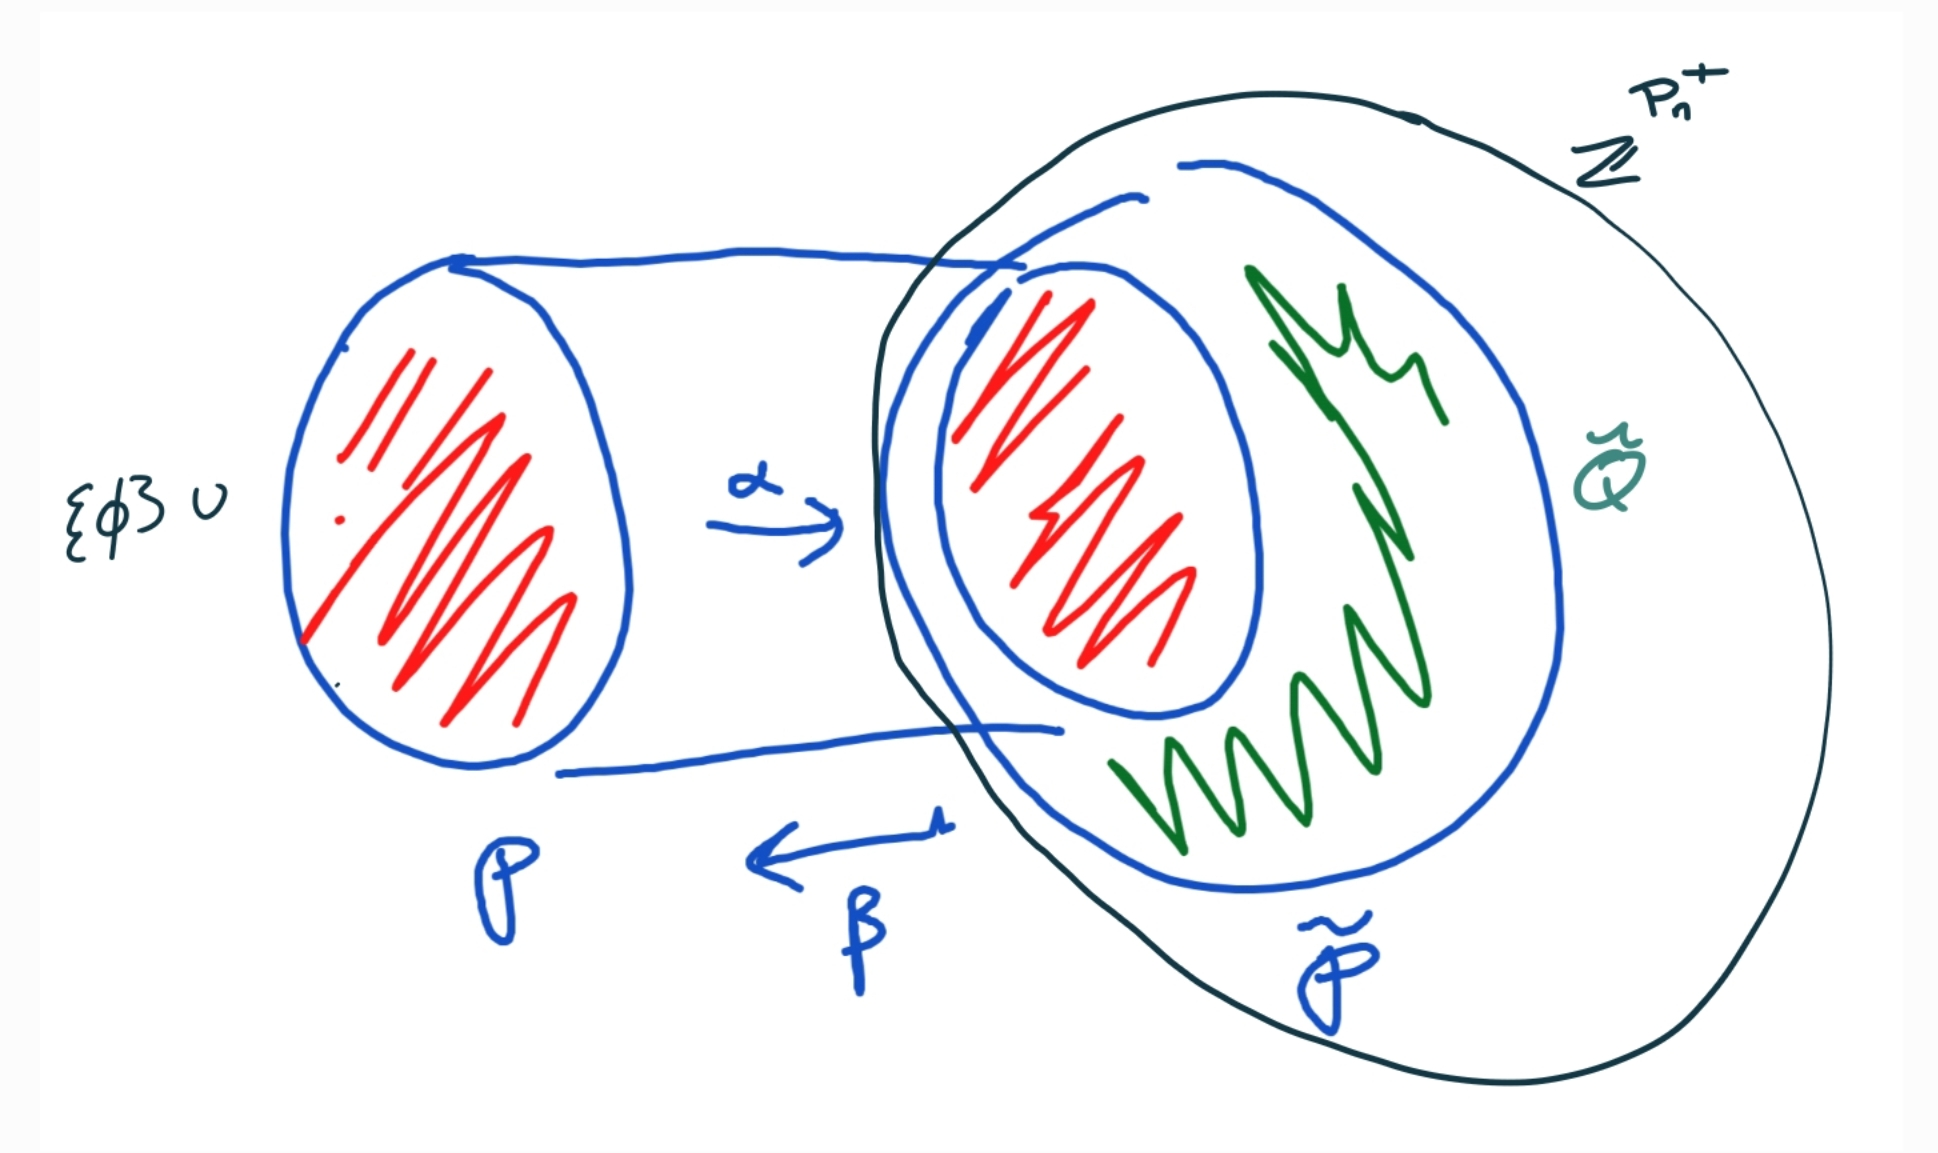
\includegraphics[scale=0.15,angle=0]{29072020 pics/3alphabeta.jpg}  
    \caption{}
    \label{relation}
\end{figure}

 

 
     There exists a map $\mathbb{Z}^{ 2^{[n]} \setminus \{\emptyset\}}  \rightarrow  \emptyset \cup P_{n}$, where $\tilde{P_n}   \subseteq \mathbb{Z}^{ 2^{[n]}\setminus \{\emptyset\} }$ (the set $\mathbb{Z}^{ 2^{[n]} \setminus \{\emptyset\}}$ has no mildly super additive condition).
     
     \begin{lemma}\label{emptymapto}
     If $f \in \mathbb{Z}^{ 2^{[n]} \setminus \{\emptyset\}}  \setminus \tilde{P_n}$ then $R_f=\emptyset$.
     \end{lemma}
     
     \begin{proof}
            
        Let $f \in \mathbb{Z}^{ 2^{[n]} \setminus \{\emptyset\}}  \setminus \tilde{P_n}$. Consider the definition of $R_f$ for $f(I)$,
        
        \begin{equation}\label{1set}
            f(I) < X_I < f(I) +1.
        \end{equation}
        
  As $f$ is not MSA let
        $$f(I \sqcup J)= f(I) + f(I) +p$$
        
        for $p \ne 0,1 \in \mathbb{Z}$ and consider
     
     
      $$f(I \sqcup J) < X_{I \sqcup J} < f(I \sqcup J) +1, $$
      which is equivalent to 
     \begin{align} \label{pterm}
   f(I) + f(J) +p < X_I + X_J < f(I) + f(J) +p +1.
     \end{align}
 
       multiply inequality (\ref{1set}) by $-1$ to give 

$$ -f(I) -1 < -X_I < -f(I),$$

and sum this with inequality (\ref{pterm}) to give

\begin{equation} \label{pinequal}
    f(I) + p -1 < X_J <  f(I) +p +1.
\end{equation}


Consider the intersection of the region given by (\ref{pinequal}) with region (\ref{1set}) for $p \ne 0,1$. This shows $R_f=\emptyset$. 

     \end{proof}
     
 
 \begin{problem}
   Show $\beta \mid _{\tilde{P_n}\setminus \tilde{Q}} $and $\alpha$ are inverses for $n<5$.
 \end{problem}

\begin{attempt} (NOT HYPERCUBE CASE, this is infinite case).

\end{attempt}

 \begin{problem}
   Show $\beta \mid _{\tilde{P_n}\setminus \tilde{Q}} $ and $\alpha$ are inverses for all $n$.
 \end{problem}
 
  Q: Since we have removed the empty set possibility will it work in generality? 
 
 \begin{attempt}
 
 First we show $\beta \mid _{\tilde{P_n}\setminus \tilde{Q}}(\alpha(R))=R$. Fix an $R \in P_n= \mathbb{R}^n \setminus H(S,k)$. Consider $\alpha(R)= c_R$ which is MSA by Lemma \ref{msamap} hence we see that $\alpha$ maps to $\tilde{P_n}\setminus \tilde{Q}$. By remark \ref{floor} note $c_{R,S}=\lfloor X_S \rfloor$ for $\underline{x} \in R$. By definition \ref{polytopes} for each choice $S \in \mathcal{P}_{n}^{+}$ we obtain $\lfloor X_S \rfloor=k$ . Consider $\beta \mid _{\tilde{P_n}\setminus \tilde{Q}}(c_R)\in P_n$ and given by, 
 
 \begin{align*}
     R_{c_R}=& \bigcap_{S \in \mathcal{P}_{n}^{+}} \{\underline{x}\in \mathbb{R}^n \mid c_{R}(S) < \sum_{i \in S} x_i < c_{R}(S)+1\}\\
     &= \bigcap_{S \in \mathcal{P}_{n}^{+}} \{\underline{x}\in \mathbb{R}^n \mid \lfloor X_S \rfloor < \sum_{i \in S} x_i < \lfloor X_S \rfloor +1\}\\
     &= \bigcap_{S \in \mathcal{P}_{n}^{+}} \{\underline{x}\in \mathbb{R}^n \mid k < \sum_{i \in S} x_i < k+1\}.\\
 \end{align*}
 
 Region $R_{c_R}$ satisfies all the definition inequalities for $R$, therefore $R_{c_R}=R$.

\begin{question}
Is $R=R_{c_R}$? 
\end{question}

\begin{attempt}

Pictorially, 
       \begin{figure}[H]
    \centering
 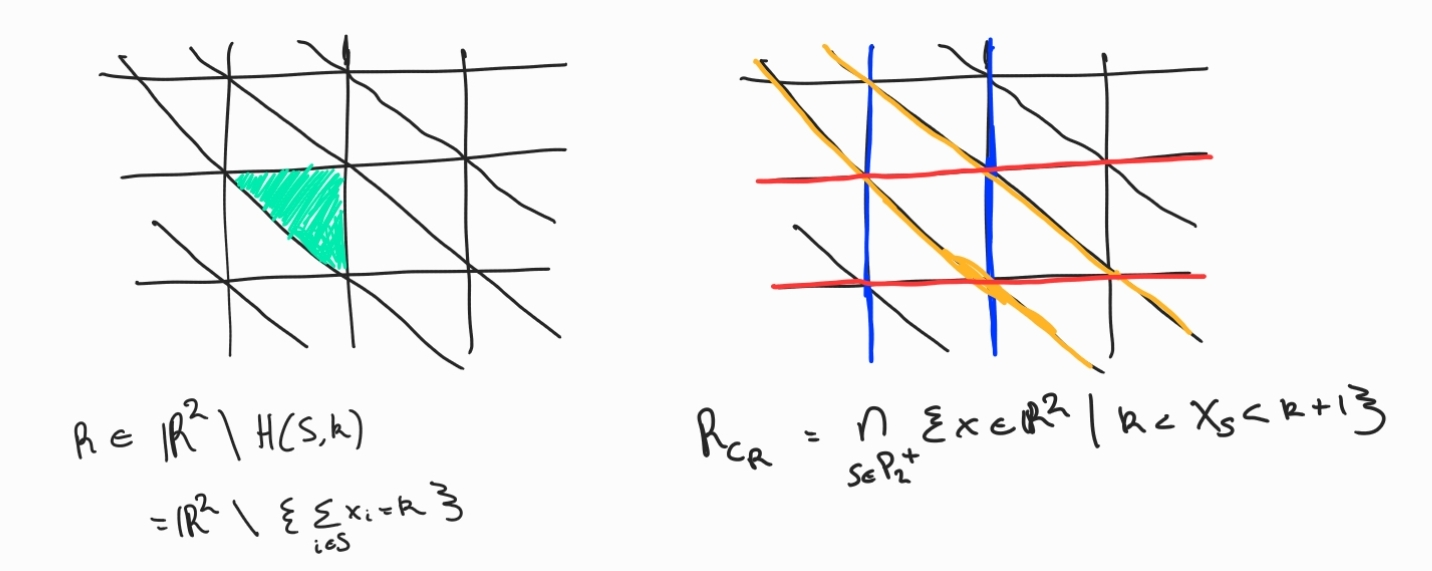
\includegraphics[scale=0.35,angle=0]{29072020 pics/RCR.jpg}  
    \caption{}
    \label{RCR}
\end{figure}

 Remark: The region $R$ is connected so every point is contained within the bounds of $H(S,k)$ for all $S$ and $k$ and does not jump over any walls so satisfies all the inequalities above.\\
 
 Show subset containment: If $\underline{x} \in R_{c_R}$ then $\underline{x}$ satisfies the inequalities for $R$, so $R_{c_R} \subseteq R$. If $\underline{x} \in R$ then $\underline{x}$ satisfies the inequalities for $R_{c_R}$.\\

Q: Is $R_{c_R}$ connected? is the intersection of connected regions connected in $\mathbb{R}^n$ (no not in general). line and circle connected but intersection not connected. MSA condition may correct. Is $R_{c_R}$ all of region $R$? Use the fact $R$ is connected/path connected.  \\
\end{attempt}


We now show $\alpha(\beta \mid _{\tilde{P_n}\setminus \tilde{Q}} (f))=f$. Consider $f \in \tilde{P_n}$ so $f$ has fixed $f(S)$ for $S \in \mathcal{P}_n^{+}$. Applying $\beta \mid _{\tilde{P_n}\setminus \tilde{Q}}$ gives a non-empty region $R_f \in P_n$ with
 
   $$R_{f}=& \bigcap_{S \in \mathcal{P}_{n}^{+}} \{\underline{x}\in \mathbb{R}^n \mid f(S) < \sum_{i \in S} x_i < f(S)+1\}.$$
 
So there exists $\underline{x} \in \mathbb{R}^n$ satisfying all the defining equations of $R_f$. 

\begin{question}
Is $c_{R_f} =f$? Does it give the same values as $f$ i.e. $f(S)=\lfloor X_S \rfloor = c_{R,S}$?
\end{question} 
 
 \begin{attempt}
 By the inequalities given in $R_f$ we have, 
 
 $$f(S) \le \lfloor X_S \rfloor < X_S < \lceil X_S \rceil \le f(S)+1 .$$
 
 \end{attempt}

Suppose $f(S)< \lfloor X_S \rfloor < X_S < \lceil X_S \rceil \le f(S)+1$, by definition of $\lfloor \: \rfloor$ and $\lceil \: \rceil$ this leads to a contradiction with the distance between $f(S)$ and $f(S)+1$. Hence $f(S)=\lfloor X_S \rfloor$ and so $\alpha(\beta \mid _{\tilde{P_n}\setminus \tilde{Q}} (f))=f$. 
  
 \end{attempt}



\subsection{Hypercube} 
    
    
We restrict our question to the hypercube. Consider the following subset. 
            $$P_n ^{'} = \{ c \in P_n \mid c \subseteq [0,1]^n\} \subseteq  P_n$$
            
            \begin{problem}
             In $\tilde{P_n}$ what is the image of $\alpha(P_n ^{'})$.
            \end{problem}
            
            The hypercube can be realised in $\tilde{P_n}$ by $\beta$. Where the hypercube is given by setting the function value for singletons to be $f(\{i\})=0$.

            
            $$\tilde{P_n}^{'} = \{ f \in  \tilde{P_{n}} \mid  f (\{ i \})=0 \quad \text{ s.t }  0 \le i\le n \} \subseteq \tilde{P_n}$$
            
            \begin{problem}
              In $P_n$ what is the image of $\beta(\tilde{P_n}^{'})$ and $\beta \mid _{\tilde{P_n}\setminus \tilde{Q}}(\tilde{P_n}^{'})$.
            \end{problem}
    
    When we say we restrict our study to the hypercube, we mean to restrict to the maps $\alpha \mid_{P_n ^{'}} : P_n ^{'} \rightarrow \tilde{P_n}^{'}$ and  $\beta \mid _{\tilde{P_n}^{'}} : \tilde{P_n}^{'} \rightarrow P_{n}^{'} \cup \{\emptyset\}$. 
    
 \begin{problem}
   Show that when we restrict to the hypercube the maps $\beta \mid _{\tilde{P_n}^{'}\setminus \tilde{Q}} $and $\alpha$ are inverses for $n<5$ .
 \end{problem}

\begin{proof}
    For $n=2,3$ we visualise the regions and prescribe $f \in \tilde{P_2},\tilde{P_3}$ with values and conclude this to be a bijection. Here we do $\alpha$ then $\beta$. See Counting hypercube regions file.
    
    To avoid the difficulty in visualisation, for the $n=4$ case we do $\beta$ then $\alpha$. See Google sheets file MSA Functions. Given the condition $f({i})=0$, we determine all the cases for $f(I)$ using the MSA condition.
    
    The MSA file data is as follows: For $n=3$ there is a choice for the value on $2$-sets e.g $\{1,2\}$. We permute through all possible choices. For a given permutation e.g. $f(\{1,2\})=1,f(\{1,3\})=0,f(\{2,3\})=0$ and consider $f(\{I \sqcup J\})$ for $J$ a $1$-set. To determine all values for a general $n$, the set $J$ will be a $n-r$ -set for $I$ an $r$-set. To make sure we have all possible decomposition's as disjoint unions its important to note that $3=1+2$, $4=1+3=2+2$ and $5=1+4=2+3$ and in general for $n$ even/odd there are $n/2$ , $\lfloor n/2 \rfloor$ ways to decompose into disjoint unions.
\end{proof}

\printindex

\bibliographystyle{alpha}
\bibliography{bibtex}



\end{document}


